\documentclass{article}
\usepackage[margin=2.5cm]{geometry}
\usepackage{enumerate, fancyhdr, graphicx, amsmath}

\title{Old School Tetris Meets Game Tree Search}
\author{Paul Chesnais (pmc85) and Sam Svenningsen (sjs382)}
\date{\today}

\pagestyle{fancy}
\fancyhead{}
\lhead{pmc85 and sjs382}
\chead{PRAC CS 4700 - Proposal}
\rhead{\today}
\fancyfoot{}
\rfoot{\thepage}
\lfoot{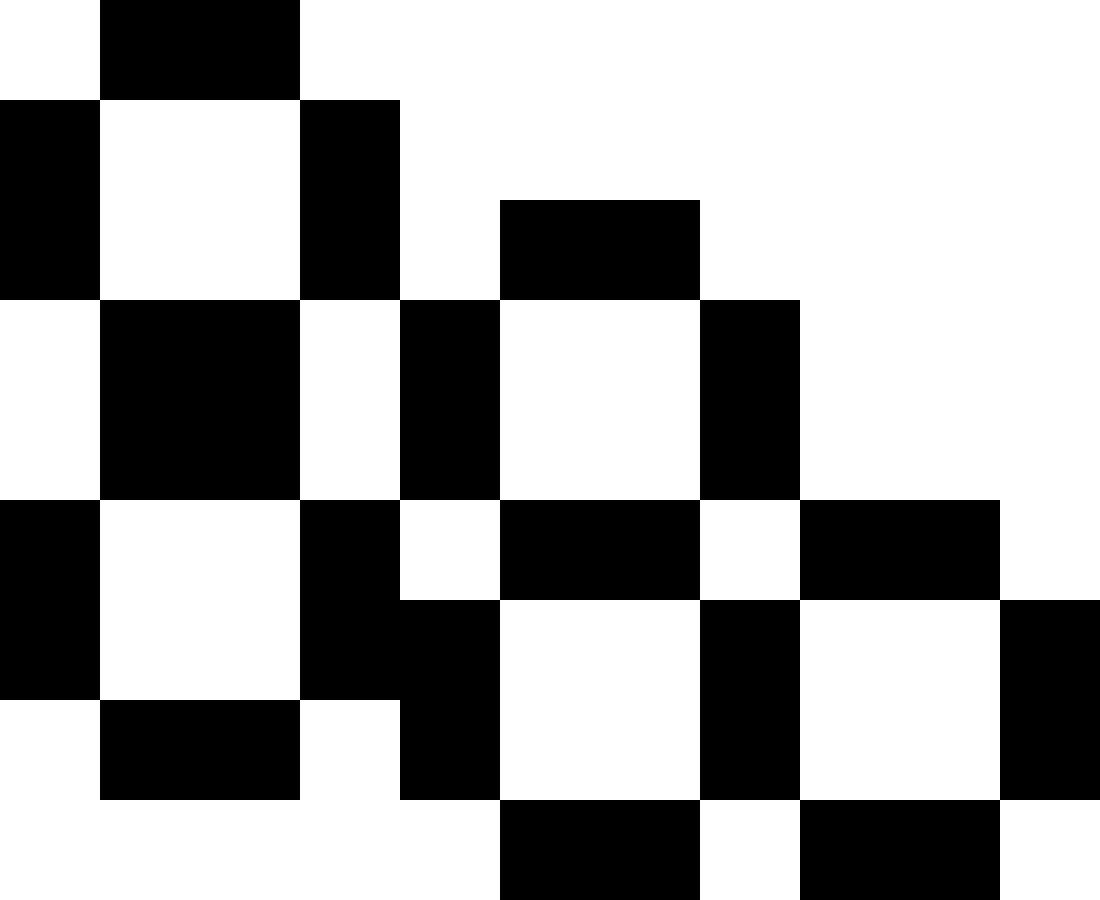
\includegraphics[height=20pt]{Logo}}
\renewcommand{\headrulewidth}{0.5pt}
\renewcommand{\footrulewidth}{0.5pt}

\def\tetris{Tetris\textsuperscript{\textregistered}}

\newcommand{\exo}[1]{\section*{Exercise #1}}
\newcommand{\prob}[1]{\section*{Problem #1}}
\newcommand{\quest}[1]{\section*{Question #1}}
\newcommand{\e}{&=&}
\newcommand{\p}[1]{\times 10^{#1}}

\begin{document}
\maketitle
\thispagestyle{empty}

\section{Description}

\par For our Project in the AI Practicum, we plan on building a \tetris{} bot. Ideally, this bot would play at speeds far greater than normal human speed, and if at all possible, when faced with the original implementation of \tetris{}, would beat the current human world record.

\section{Approach}



\section{Plan}

Try different approaches to compare success and easiness. Success being average score and max highest score with each approach.

\begin{description}

  \item[Graph Traversal (Look for actual name)] Calculate all possibilities n moves ahead, choose best. Best being a ``perfect'' Tetris stack (i.e. no holes) for as many consecutive pieces as possible.

  \item[Heuristic Approach] Find out if we can get a heuristic function that gives a score to a tetris state plus a new piece or pieces in any configuration and choose the max (or min) value one.

  \item[A* search]

  \item[Reinforcement Learning]?

\end{description}


\section{Timeline}



\end{document}
